\documentclass[10pt]{article}
\usepackage{graphicx} % Required for inserting images
\usepackage[margin=0.8in]{geometry}
\usepackage[T1]{fontenc}
\usepackage{amsmath}
\usepackage{booktabs}
\usepackage{float}
\usepackage{enumitem}
\usepackage{hyperref}

\setlist{itemsep=2pt, topsep=3pt}
\setlength{\textfloatsep}{8pt plus 2pt minus 2pt}
\setlength{\floatsep}{8pt plus 2pt minus 2pt}
\setlength{\intextsep}{8pt plus 2pt minus 2pt}
\setlength{\abovecaptionskip}{4pt}

\begin{document}

\begin{center}
{\Large Deep Averaging Networks $|$ Byte Pair Encoding $|$ Skip-Gram}\\[6pt]
Thanh Trinh - TSS: 200197841
\end{center}


\section{Methods and Experimental Setup}

\subsection{Approach}

I started from the provided bag-of-words pipeline (about 0.71 dev accuracy) and kept its training loop, loss and
evaluation, changing only the input representation and the model. The plan was to (1) build a word-level DAN on
pretrained GloVe embeddings and tune it well past 77\%, (2) change one design choice at a time to see which ones
matter (1a), (3) replace GloVe with randomly initialized embeddings (1b), and (4) replace word tokens with BPE
subwords (Part 2). Steps 3 and 4 use the same classifier and training setup, so accuracy differences come from the
input representation alone. Part 3 was solved analytically, and the answers were checked numerically.

Going into this assignment, I thought most of the work would be building and tuning the model, but the model itself
was fairly straightforward. Most of my time went into handling the input representations and making them work with
the existing training code.

\subsection{Implementation}

\paragraph{DAN (\texttt{DANmodels.py}).} Each sentence becomes a list of token indices (unknown words map to
\texttt{UNK}, whose GloVe vector starts at zero), padded with \texttt{PAD} (index 0) within a batch. The embeddings
are averaged over real tokens only, using a padding mask, so the representation does not depend on how much padding
the batch needs. The average goes through dropout, then hidden layers (Linear $\to$ ReLU $\to$ dropout), then a
Linear layer to 2 classes and a log-softmax, trained with \texttt{NLLLoss}. The embedding layer comes from
\texttt{get\_initialized\_embedding\_layer(frozen=False)}, so GloVe is fine-tuned. I also implemented the
\emph{word dropout} of Iyyer et al.: during training each token is removed from the average with probability $p$,
but at least one token per sentence is always kept.

\paragraph{BPE (\texttt{bpe.py}).} Following Sennrich et al., each training word is split into characters, with an
end-of-word marker attached to the last one (\texttt{low} $\to$ \texttt{l o w</w>}) so suffixes are distinguished
from word pieces. The most frequent adjacent pair (weighted by word frequency) is merged repeatedly until the
vocabulary reaches the target size, or until no pair occurs twice (at 13,368 tokens on \texttt{train.txt},
counting \texttt{PAD} and \texttt{UNK}). Pair counts are updated incrementally, touching only words that contain the
merged pair, so a 10,000-token vocabulary (9,887 merges) takes under a second to learn. The learned merges exactly match a naive implementation that recounts every pair at each step. New text is
segmented by applying the merges in the order they were learned. The subword DAN reuses the DAN above with randomly
initialized embeddings.

\paragraph{Training (\texttt{main.py}, \texttt{run\_experiments.py}).} Adam, \texttt{NLLLoss}, and train/dev loss
and accuracy printed every epoch. \texttt{run\_experiments.py} runs every experiment in this report.

\subsection{Experimental Setup}

\begin{itemize}
  \item \textbf{Data:} 6,920 training and 872 dev sentences (binary sentiment, lowercased by the provided reader).
        All results are on dev.
  \item \textbf{Training:} Adam, batch size 32, 15 epochs, on a laptop CPU. Times are training time only.
  \item \textbf{Reporting:} every configuration was run with 3 seeds. Tables report mean $\pm$ std of \emph{best}
        dev accuracy (the highest over the 15 epochs) and \emph{final} dev accuracy (after epoch 15).
  \item \textbf{Ablations:} each ablation changes one setting of a base model: fine-tuned 300d GloVe, 2 hidden
        layers of 300, ReLU, dropout 0.3, lr $10^{-3}$.
\end{itemize}

\subsection{Hyperparameters and Designs Explored}

\begin{table}[htbp]
\centering
\small
\begin{tabular}{lll}
\toprule
Setting & Values tried & Chosen \\
\midrule
Embeddings & GloVe 300d/50d, random 300d/50d & GloVe 300d \\
Embedding updates & fine-tuned, frozen & fine-tuned \\
Hidden layers $\times$ size & 1, 2, 3 layers $\times$ 100, 300 & $2 \times 300$ \\
Dropout / word dropout & 0, 0.3, 0.5 / 0, 0.3 & 0.3 / 0 \\
Learning rate & $10^{-3}$, $10^{-4}$ & $10^{-4}$ (300d GloVe), $10^{-3}$ (others) \\
BPE vocabulary size & 500, 1k, 2k, 5k, 10k, 15k & 10k \\
\bottomrule
\end{tabular}
\caption{Settings explored and the values chosen.}
\label{tab:hparams}
\end{table}

The best learning rate depends on the model. Lowering it to $10^{-4}$ is the most effective change for fine-tuning
300d GloVe (Section~\ref{sec:1a}). For 50d GloVe, $10^{-4}$ is too slow to converge in 15 epochs: a run at
$10^{-4}$ reaches only 0.753, versus $0.794 \pm 0.004$ at $10^{-3}$. \texttt{main.py} therefore defaults to
$10^{-4}$ only for the 300d GloVe DAN, and trains the 50d, random-embedding and subword models at $10^{-3}$.

\section{Results and Discussion}

\subsection{Part 1a: DAN with GloVe Embeddings}
\label{sec:1a}

\textbf{Final model:} fine-tuned 300d GloVe, 2 hidden layers of 300, ReLU, dropout 0.3, lr $10^{-4}$, 15 epochs. It
reaches \textbf{0.816 $\pm$ 0.001} final dev accuracy (0.819 best) in about 33 seconds of training, well above the
77\% target and the bag-of-words baselines (0.71 for 2 layers, 0.69 for 3 layers).

\begin{table}[htbp]
\centering
\small
\begin{tabular}{lcccc}
\toprule
Configuration & Best dev & Final dev & Final train & Time (s) \\
\midrule
Base (300d GloVe, lr $10^{-3}$) & 0.813 $\pm$ 0.000 & 0.791 $\pm$ 0.011 & 0.987 & 33 \\
\textbf{lr $\mathbf{10^{-4}}$} & \textbf{0.819 $\pm$ 0.001} & \textbf{0.816 $\pm$ 0.001} & 0.882 & 32 \\
50d GloVe & 0.803 $\pm$ 0.004 & 0.794 $\pm$ 0.004 & 0.943 & 9 \\
300d GloVe, frozen & 0.790 $\pm$ 0.001 & 0.775 $\pm$ 0.006 & 0.782 & 6 \\
50d GloVe, frozen & 0.740 $\pm$ 0.002 & 0.731 $\pm$ 0.008 & 0.674 & 4 \\
1 hidden layer & 0.817 $\pm$ 0.001 & 0.790 $\pm$ 0.002 & 0.992 & 33 \\
3 hidden layers & 0.813 $\pm$ 0.004 & 0.793 $\pm$ 0.008 & 0.987 & 35 \\
Hidden size 100 & 0.818 $\pm$ 0.002 & 0.796 $\pm$ 0.005 & 0.987 & 31 \\
No dropout & 0.816 $\pm$ 0.006 & 0.795 $\pm$ 0.010 & 0.995 & 32 \\
Dropout 0.5 & 0.818 $\pm$ 0.007 & 0.793 $\pm$ 0.010 & 0.977 & 33 \\
Word dropout 0.3 & 0.812 $\pm$ 0.001 & 0.794 $\pm$ 0.004 & 0.925 & 33 \\
\bottomrule
\end{tabular}
\caption{Part 1a ablations. Each row changes one setting of the base model (mean $\pm$ std over 3 seeds).}
\label{tab:1a}
\end{table}

\begin{figure}[htbp]
\centering
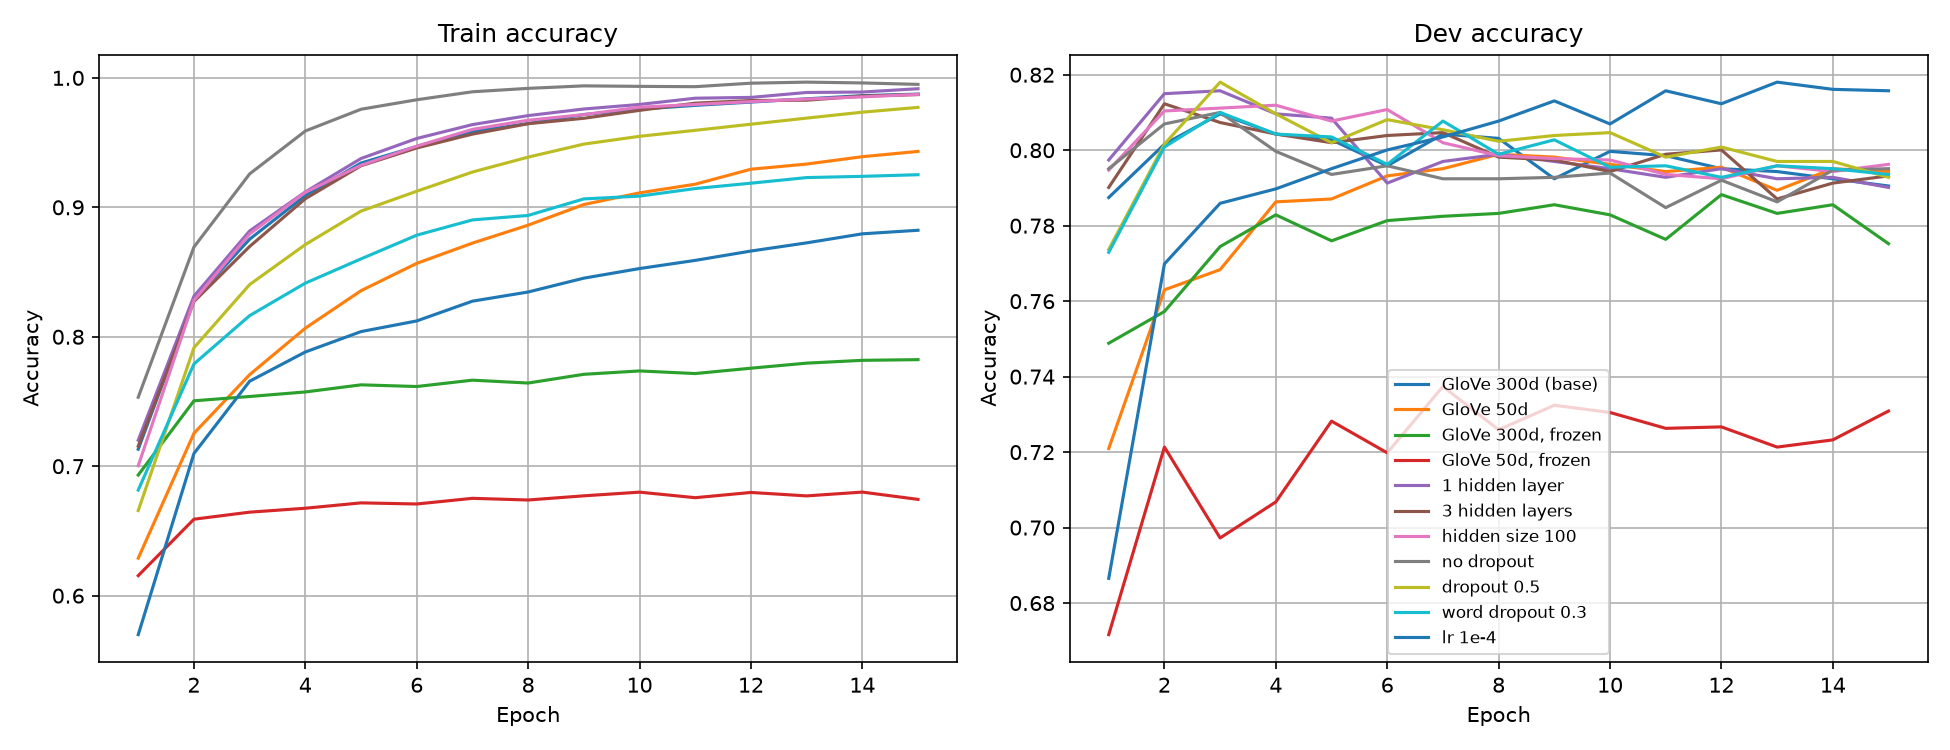
\includegraphics[width=0.92\linewidth]{results/part1a_curves.png}
\caption{Part 1a train and dev accuracy per epoch (mean over 3 seeds).}
\label{fig:1a}
\end{figure}

\paragraph{Observations.}
\begin{itemize}
  \item \textbf{Every fine-tuned configuration clears 77\%.} The DAN beats the bag-of-words baseline by about 10
        points, because pretrained embeddings let it generalize to words that are rare in the 6,920 training
        sentences.
  \item \textbf{Overfitting is the main issue.} At lr $10^{-3}$ dev accuracy peaks within 2--6 epochs and then
        declines while training accuracy approaches 99\%. The embedding matrix (about 4.5M parameters at 300d) can
        memorize the small training set. Lowering the learning rate to $10^{-4}$ was the most effective change: dev
        accuracy rises steadily and stays near its peak (best 0.819, final 0.816, with the lowest variance across
        seeds).
  \item \textbf{Fine-tuning matters.} Freezing the embeddings costs 2.3 points at 300d and 6.3 points at 50d.
        Frozen models underfit (final train accuracy 0.67--0.78): GloVe's general-purpose vectors are not tuned for
        sentiment, for example ``good'' and ``bad'' have similar contexts and therefore similar vectors. 300d is more
        robust than 50d, especially when frozen, since the extra dimensions leave more room for sentiment-relevant
        directions.
  \item \textbf{Architecture changes have little effect.} Depth (1--3 layers), hidden size (100 vs.\ 300) and
        standard dropout (0--0.5) all move best dev accuracy by under 0.6 points, within about one standard
        deviation. Dropout and word dropout reduce training accuracy (word dropout: 0.925 vs.\ 0.987) but do not
        improve dev accuracy at lr $10^{-3}$, because the overfitting comes mostly from the embedding updates.
\end{itemize}

What surprised me most was that adding hidden layers or dropout barely changed accuracy, while simply lowering the
learning rate helped the most. Seeing training accuracy near 99\% while dev accuracy dropped showed me that fitting
the training data better does not mean performing better on unseen data.

\subsection{Part 1b: Randomly Initialized Embeddings}

For random initialization, the vocabulary is built from the training set (\texttt{PAD}, \texttt{UNK} and every
training word, 14,832 types) and the embeddings are drawn from $\mathcal{N}(0, 1)$ by \texttt{nn.Embedding}. Dev
words that never appear in training (5.7\% of dev tokens) map to \texttt{UNK}; otherwise their random vectors would
never be updated and would add pure noise to the average. Everything else matches the base model (lr $10^{-3}$, 15
epochs).

\begin{table}[htbp]
\centering
\small
\begin{tabular}{lcccc}
\toprule
Embeddings & Best dev & Final dev & Final train & Epoch of best dev \\
\midrule
GloVe 300d & 0.813 $\pm$ 0.000 & 0.791 $\pm$ 0.011 & 0.987 & 5.7 \\
Random 300d & 0.786 $\pm$ 0.004 & 0.783 $\pm$ 0.003 & 0.977 & 10.7 \\
GloVe 50d & 0.803 $\pm$ 0.004 & 0.794 $\pm$ 0.004 & 0.943 & 9.0 \\
Random 50d & 0.776 $\pm$ 0.012 & 0.771 $\pm$ 0.013 & 0.914 & 14.7 \\
\bottomrule
\end{tabular}
\caption{GloVe vs.\ randomly initialized embeddings (mean $\pm$ std over 3 seeds).}
\label{tab:1b}
\end{table}

\begin{figure}[htbp]
\centering
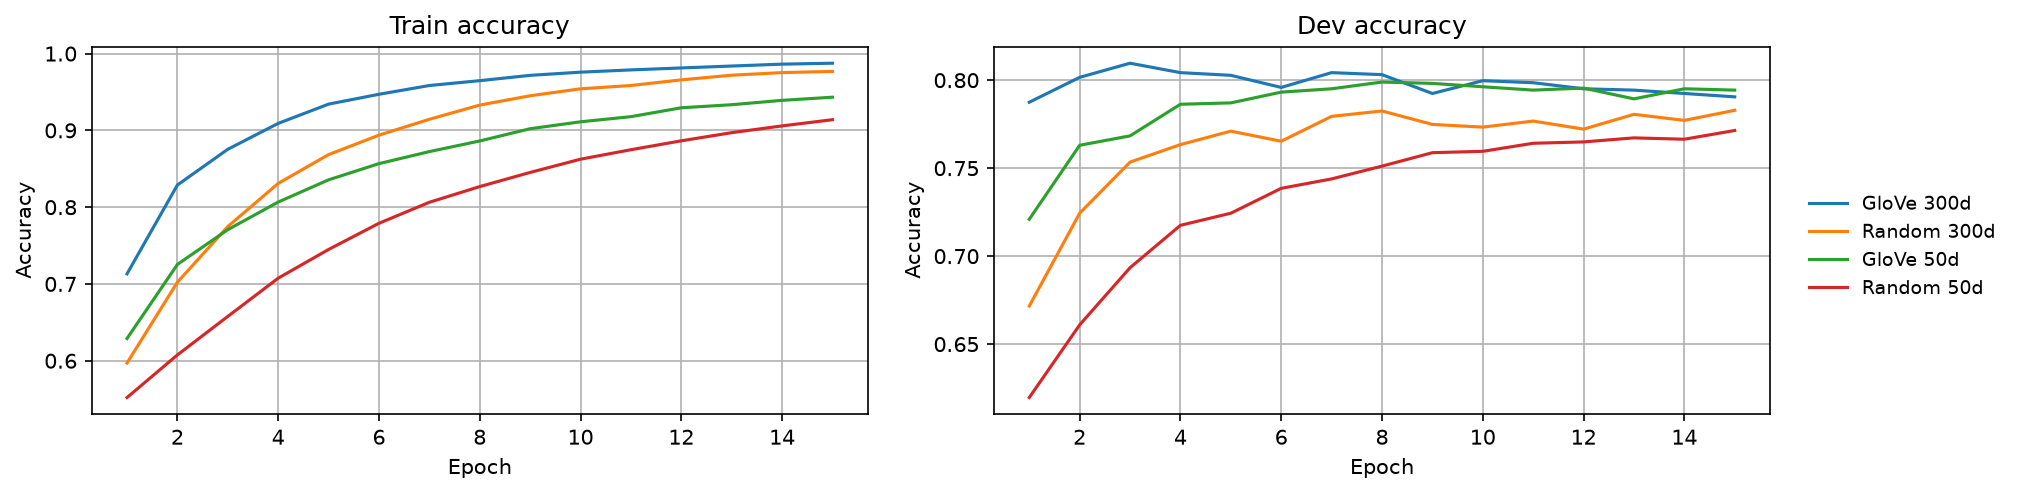
\includegraphics[width=0.92\linewidth]{results/part1b_curves.png}
\caption{Part 1b train and dev accuracy per epoch (mean over 3 seeds).}
\label{fig:1b}
\end{figure}

Random embeddings still reach about 78--79\% at 300d (just above the 77\% target), but they are 2.7 points worse
than GloVe at the peak, and the effect on convergence is clear:
\begin{itemize}
  \item \textbf{Slower convergence.} With GloVe the first epoch already gives about 76\% dev accuracy, because
        similar words start with similar vectors and the network only has to learn a classifier on top. With random
        vectors every word starts unrelated to every other, and sentiment information has to reach each embedding
        through the gradients of the sentences it appears in. Best dev accuracy arrives at epoch 10.7 instead of 5.7
        (300d), and at 50d the model is still improving at epoch 15.
  \item \textbf{Worse generalization.} A word seen once or twice in training gets only a few noisy updates, and
        unseen dev words collapse to \texttt{UNK}. GloVe carries information learned from billions of tokens, so
        rare and unseen-in-train words still contribute a useful signal.
  \item \textbf{Higher variance.} Random 50d has $3\times$ the seed-to-seed standard deviation of GloVe 50d.
\end{itemize}

\subsection{Part 2a: Subword DAN with BPE}

The subword DAN uses randomly initialized 300d embeddings, lr $10^{-3}$, 15 epochs (BPE implementation in
Section~1.2). Example segmentation with vocabulary size 2000: \texttt{unbelievably overwrought} $\to$
\texttt{un believ ably</w> over wr ought</w>}.

\begin{table}[htbp]
\centering
\small
\begin{tabular}{lccccc}
\toprule
Model & Vocab & Tokens/sent. & Best dev & Final dev & Time (s) \\
\midrule
Word-level DAN, random 300d & 14,832 & 19.3 & 0.786 $\pm$ 0.004 & 0.783 $\pm$ 0.003 & 32 \\
Word-level DAN, GloVe 300d (1a) & 14,923 & 19.3 & 0.819 $\pm$ 0.001 & 0.816 $\pm$ 0.001 & 32 \\
\midrule
BPE 500 & 502 & 42.3 & 0.713 $\pm$ 0.004 & 0.693 $\pm$ 0.002 & 9 \\
BPE 1000 & 1,002 & 35.2 & 0.747 $\pm$ 0.006 & 0.713 $\pm$ 0.011 & 10 \\
BPE 2000 & 2,002 & 29.9 & 0.761 $\pm$ 0.003 & 0.747 $\pm$ 0.014 & 11 \\
BPE 5000 & 5,002 & 24.7 & 0.779 $\pm$ 0.007 & 0.761 $\pm$ 0.002 & 17 \\
BPE 10000 & 10,002 & 21.8 & 0.784 $\pm$ 0.006 & 0.779 $\pm$ 0.005 & 25 \\
BPE 15000 (all merges) & 13,368 & 20.8 & 0.786 $\pm$ 0.002 & 0.770 $\pm$ 0.005 & 32 \\
\bottomrule
\end{tabular}
\caption{Subword DAN at different BPE vocabulary sizes vs.\ word-level DANs (mean $\pm$ std over 3 seeds).}
\label{tab:2a}
\end{table}

\begin{figure}[htbp]
\centering
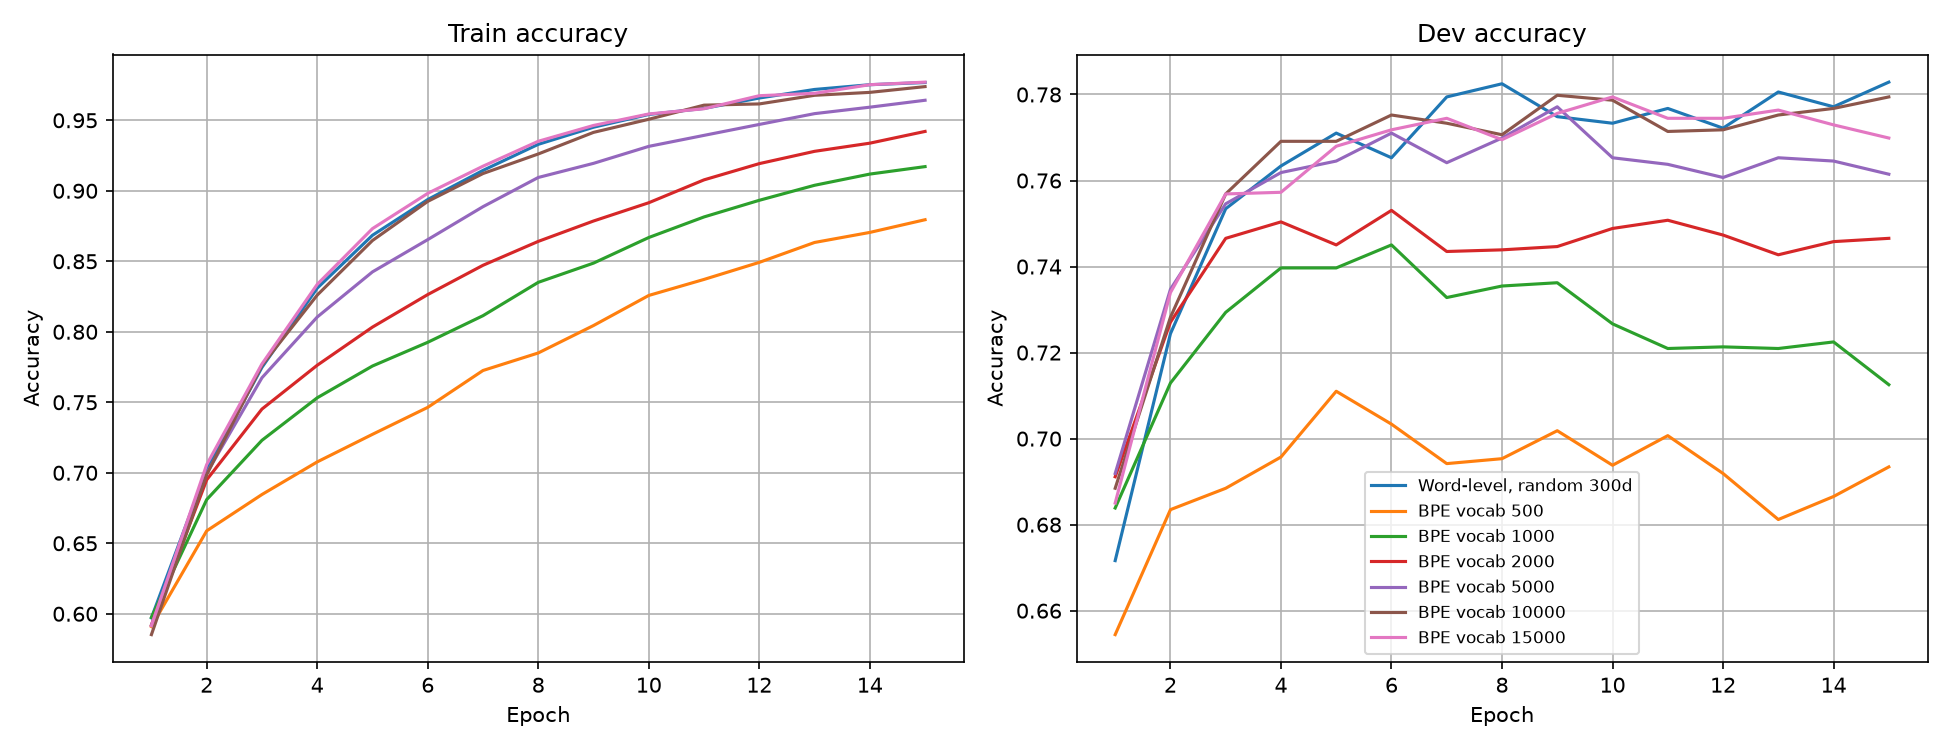
\includegraphics[width=0.92\linewidth]{results/part2_curves.png}
\caption{Part 2 train and dev accuracy per epoch (mean over 3 seeds).}
\label{fig:2a}
\end{figure}

\begin{itemize}
  \item \textbf{Accuracy increases with vocabulary size.} Accuracy rises from 0.713 at 500 subwords to
        0.784--0.786 at 10k--13k, which matches the word-level DAN with random embeddings (0.786). Small
        vocabularies break words into short fragments (42 tokens per sentence at 500, versus 19 words). With 500
        subwords, ``brilliant'' becomes \texttt{br il li ant</w>} and ``masterpiece'' becomes
        \texttt{ma st er pi ec e</w>}. Since a DAN averages its inputs without word order, it cannot recombine such
        fragments into the meaning of the whole word. Fragments shared by many unrelated words carry little
        sentiment of their own, and averaging dilutes the informative ones.
  \item \textbf{Large vocabularies converge to word level.} At 10k+ merges almost every frequent word is a single
        token, so the model behaves like the word-level DAN. The subword model never beats word level on this data,
        but it gets close with fewer parameters (10k vs.\ 14.8k embeddings).
  \item \textbf{BPE removes unknown words.} The word-level model maps 5.7\% of dev tokens to \texttt{UNK}, while BPE
        segments almost everything into known pieces (only 3 dev tokens contain unseen characters). On this
        in-domain data the benefit is small, since most OOV words are numbers and names (\texttt{1873},
        \texttt{87-minute}, \texttt{abrams}) that carry little sentiment.
  \item \textbf{Efficiency trade-off.} A smaller vocabulary means a smaller embedding table ($500 \times 300 =$
        150k parameters vs.\ 4M at 13k) and much faster training (9s vs.\ 32s for 15 epochs, since the dense
        embedding gradient and Adam update touch the whole table every step), even though sentences become twice as
        long. Training BPE itself is negligible ($<$1s).
  \item \textbf{Neither matches GloVe.} All random-initialization models trail the GloVe DAN (0.816) by 3+ points.
        Pretraining matters more than the choice of token unit on a dataset this small.
\end{itemize}

I would choose a vocabulary size of around 10,000: it nearly matched the word-level model with fewer embeddings and
less training time, while very small vocabularies trained faster but lost a lot of accuracy.

\section{Part 3: Understanding Skip-Gram}

\subsection*{Q1}

With window $k = 1$, the sentences ``the dog'', ``the cat'', ``a dog'' give the training pairs
(the, dog), (dog, the), (the, cat), (cat, the), (a, dog), (dog, a).

\paragraph{3a)} The center word \emph{the} appears in two training examples, with contexts \emph{dog} and
\emph{cat}. Maximum likelihood matches the empirical distribution, so
\[
P(\text{dog} \mid \text{the}) = \tfrac12, \quad P(\text{cat} \mid \text{the}) = \tfrac12, \quad
P(\text{a} \mid \text{the}) = 0, \quad P(\text{the} \mid \text{the}) = 0.
\]

\paragraph{3b)} Yes. The context vectors are $c_{\text{dog}} = c_{\text{cat}} = (0, 1)$ and
$c_{\text{a}} = c_{\text{the}} = (1, 0)$. Take $\mathbf{v_{\text{the}} = (0, 10)}$, so
$v_{\text{the}} \cdot c_{\text{dog}} = v_{\text{the}} \cdot c_{\text{cat}} = 10$ and
$v_{\text{the}} \cdot c_{\text{a}} = v_{\text{the}} \cdot c_{\text{the}} = 0$. Then
\[
P(\text{dog} \mid \text{the}) = P(\text{cat} \mid \text{the}) = \frac{e^{10}}{2e^{10} + 2e^{0}}
= \frac{22026.5}{44055} \approx \mathbf{0.49998}, \qquad
P(\text{a} \mid \text{the}) = P(\text{the} \mid \text{the}) = \frac{1}{44055} \approx \mathbf{0.00002},
\]
which are within 0.01 of the optimum $(\tfrac12, \tfrac12, 0, 0)$.

\emph{Why it is optimal:} the target puts equal mass on \emph{dog} and \emph{cat}, which share a context vector, so
any $v_{\text{the}}$ automatically scores them equally. The only remaining goal is to make \emph{a} and \emph{the}
negligible, which means making the second coordinate of $v_{\text{the}}$ much larger than the first. As the scale
grows ($v_{\text{the}} = (0, t)$, $t \to \infty$), the probabilities approach exactly $(\tfrac12, \tfrac12, 0, 0)$.
The exact optimum needs infinite weights; $t = 10$ already gets within $2 \times 10^{-5}$. (Any $t \geq 4$ gets
within 0.01; $v_{\text{the}} = (-10, 10)$ is even closer.)

\subsection*{Q2}

\paragraph{3c)} Sentences ``the dog'', ``the cat'', ``a dog'', ``a cat'' with $k = 1$ give 8 training examples
$(x, y)$:
\[
(\text{the}, \text{dog}),\ (\text{dog}, \text{the}),\ (\text{the}, \text{cat}),\ (\text{cat}, \text{the}),\
(\text{a}, \text{dog}),\ (\text{dog}, \text{a}),\ (\text{a}, \text{cat}),\ (\text{cat}, \text{a})
\]

\paragraph{3d)} The empirical (optimal) conditionals are
$P(\text{dog} \mid \text{the}) = P(\text{cat} \mid \text{the}) = P(\text{dog} \mid \text{a}) = P(\text{cat} \mid
\text{a}) = \tfrac12$ and $P(\text{the} \mid \text{dog}) = P(\text{a} \mid \text{dog}) = P(\text{the} \mid
\text{cat}) = P(\text{a} \mid \text{cat}) = \tfrac12$, with all other probabilities 0. Determiners predict nouns
and nouns predict determiners, so we put the two groups on orthogonal axes:

\begin{table}[H]
\centering
\small
\begin{tabular}{lcc}
\toprule
Word & Word vector $v$ & Context vector $c$ \\
\midrule
the & $(0, 10)$ & $(1, 0)$ \\
a & $(0, 10)$ & $(1, 0)$ \\
dog & $(10, 0)$ & $(0, 1)$ \\
cat & $(10, 0)$ & $(0, 1)$ \\
\bottomrule
\end{tabular}
\caption{Word and context vectors that nearly optimize the skip-gram objective.}
\label{tab:3d}
\end{table}

\paragraph{Check.}
\begin{itemize}
  \item $v_{\text{the}} \cdot c_{\text{dog}} = v_{\text{the}} \cdot c_{\text{cat}} = 10$ and
        $v_{\text{the}} \cdot c_{\text{the}} = v_{\text{the}} \cdot c_{\text{a}} = 0$, so
        $P(\text{dog} \mid \text{the}) = P(\text{cat} \mid \text{the}) = e^{10} / (2e^{10} + 2) \approx 0.49998$
        and $P(\text{the} \mid \text{the}) = P(\text{a} \mid \text{the}) \approx 0.00002$. The same holds for
        \emph{a}.
  \item $v_{\text{dog}} \cdot c_{\text{the}} = v_{\text{dog}} \cdot c_{\text{a}} = 10$ and
        $v_{\text{dog}} \cdot c_{\text{dog}} = v_{\text{dog}} \cdot c_{\text{cat}} = 0$, so
        $P(\text{the} \mid \text{dog}) = P(\text{a} \mid \text{dog}) \approx 0.49998$ and
        $P(\text{dog} \mid \text{dog}) = P(\text{cat} \mid \text{dog}) \approx 0.00002$. The same holds for
        \emph{cat}.
\end{itemize}

Every conditional is within $2 \times 10^{-5}$ of the optimum (well within 0.01), so these vectors nearly maximize
the skip-gram objective. Scaling $10 \to \infty$ approaches the exact optimum. I also verified these probabilities
numerically.

\end{document}
